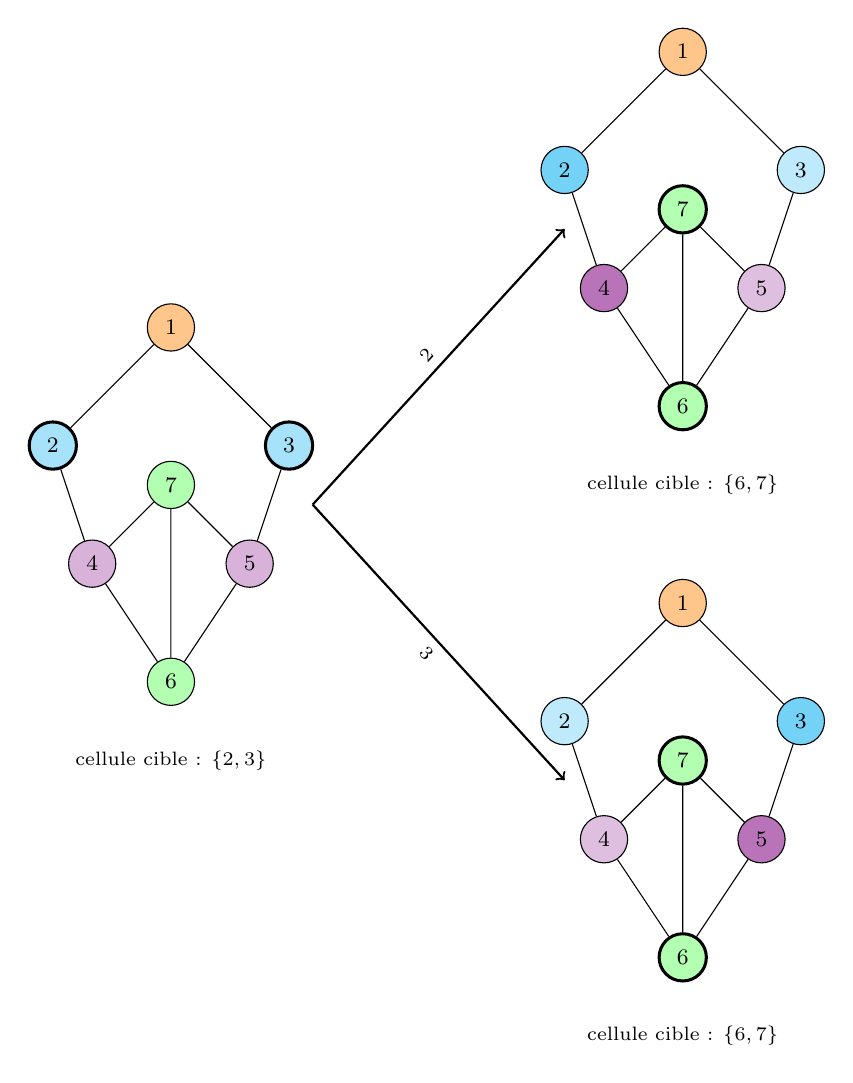
\begin{tikzpicture}
      \tikzset{v/.style={circle, draw, minimum size=6mm, inner sep=0pt, font=\footnotesize}}
      \tikzset{vt/.style={v, line width=1.1pt}}
      
      % ---- Root (gauche) : cellule cible {2,3} mise en evidence ----
      \begin{scope}[xshift=0cm, yshift=0cm]
      \node[v, fill=orange!45] (r1) at (0,2.5) {1};
      \node[vt, fill=cyan!35] (r2) at (-1.5,1) {2};
      \node[vt, fill=cyan!35] (r3) at (1.5,1) {3};
      \node[v, fill=violet!30] (r4) at (-1,-0.5) {4};
      \node[v, fill=violet!30] (r5) at (1,-0.5) {5};
      \node[v, fill=green!30] (r6) at (0,-2) {6};
      \node[v, fill=green!30] (r7) at (0,0.5) {7};
      \draw (r1)--(r2) (r1)--(r3) (r2)--(r4) (r3)--(r5)
            (r4)--(r6) (r5)--(r6) (r4)--(r7) (r5)--(r7) (r6)--(r7);
      \node[align=center, font=\scriptsize] at (0,-3) {cellule cible : $\{2,3\}$};
      \end{scope}
      
      % ---- Enfant haut (droite) : individualiser 2 ----
      \begin{scope}[xshift=6.5cm, yshift=3.5cm]
      \node[v, fill=orange!45] (l1) at (0,2.5) {1};
      \node[v, fill=cyan!55] (l2) at (-1.5,1) {2};
      \node[v, fill=cyan!25] (l3) at (1.5,1) {3};
      \node[v, fill=violet!55] (l4) at (-1,-0.5) {4};
      \node[v, fill=violet!25] (l5) at (1,-0.5) {5};
      \node[vt, fill=green!30] (l6) at (0,-2) {6};
      \node[vt, fill=green!30] (l7) at (0,0.5) {7};
      \draw (l1)--(l2) (l1)--(l3) (l2)--(l4) (l3)--(l5)
            (l4)--(l6) (l5)--(l6) (l4)--(l7) (l5)--(l7) (l6)--(l7);
      \node[align=center, font=\scriptsize] at (0,-3) {cellule cible : $\{6,7\}$};
      \end{scope}
      
      % ---- Enfant bas (droite) : individualiser 3 ----
      \begin{scope}[xshift=6.5cm, yshift=-3.5cm]
      \node[v, fill=orange!45] (s1) at (0,2.5) {1};
      \node[v, fill=cyan!25] (s2) at (-1.5,1) {2};
      \node[v, fill=cyan!55] (s3) at (1.5,1) {3};
      \node[v, fill=violet!25] (s4) at (-1,-0.5) {4};
      \node[v, fill=violet!55] (s5) at (1,-0.5) {5};
      \node[vt, fill=green!30] (s6) at (0,-2) {6};
      \node[vt, fill=green!30] (s7) at (0,0.5) {7};
      \draw (s1)--(s2) (s1)--(s3) (s2)--(s4) (s3)--(s5)
            (s4)--(s6) (s5)--(s6) (s4)--(s7) (s5)--(s7) (s6)--(s7);
      \node[align=center, font=\scriptsize] at (0,-3) {cellule cible : $\{6,7\}$};
      \end{scope}
      
      % ---- Fleches ----
      \draw[->, thick] (1.8,0.25) -- node[above, sloped, font=\scriptsize] {$2$} (5.0,3.75);
      \draw[->, thick] (1.8,0.25) -- node[below, sloped, font=\scriptsize] {$3$} (5.0,-3.25);
      
      \end{tikzpicture}